\chapter{Apéndice}
\label{ap:medicion_alta_impedancia}

Durante la formulación del proyecto se analizó la posibilidad de diseñar un
circuito propio para la medición de la resistencia del cuerpo a tierra con una
precisión objetivo de $\pm 15\%$. Sin embargo, debido a las limitaciones de
tiempo y al alcance definido para el proyecto, se decidió utilizar un probador
comercial como subsistema principal de verificación ESD.

El dispositivo seleccionado es capaz de medir resistencias de cuerpo a tierra en
un rango aproximado de 750 k$\Omega$ a 10 M$\Omega$, con una precisión de
$\pm 5\%$, lo cual lo hace adecuado para la verificación de pulseras
antiestáticas de muñeca, pero no para la evaluación de calzado ESD
\cite{hzr171_oficial}. Por lo tanto, el diseño presentado en este apéndice corresponde
a un análisis complementario realizado durante la etapa de formulación. Su
implementación no forma parte de los objetivos obligatorios del proyecto ni de
los criterios principales de evaluación.

\section{Diseño de un circuito de medición de alta impedancia}

En la medición de la resistencia del usuario a tierra, sistemas industriales
portátiles como el Desco Wrist Strap Tester ofrecen una precisión de
$\pm 10\%$ para valores alrededor de 750 k$\Omega$ y de $\pm 15\%$ para
valores cercanos a 10 M$\Omega$ \cite{Desco_19240}. En el caso del sistema
industrial SmartLog Pro 2 de Desco, se reporta una precisión de $\pm 10\%$
para valores entre 750 k$\Omega$ y 35 M$\Omega$ \cite{Desco_SmartLog}. A
partir de estas referencias, se considera una precisión objetivo de
$\pm 15\%$ como un valor adecuado para un circuito experimental de medición.

Como se explicó en el Capítulo 2, la medición de resistencia puede realizarse a
partir de la ley de Ohm. Esto permite considerar dos métodos principales:
aplicar una corriente constante y medir la tensión resultante, o aplicar una
tensión constante y medir la corriente. En resistencias ideales, ambos métodos
pueden emplearse de forma directa. Sin embargo, en el caso del cuerpo humano,
la resistencia no es estrictamente constante, ya que puede variar con la
tensión, la corriente aplicada, la presión de contacto, el área de contacto y
las condiciones ambientales.

El método de corriente constante presenta una ventaja importante, ya que la
relación entre la resistencia y la tensión medida es lineal. Esta relación se
ilustra en la Figura~\ref{fig:ap_fuente_corriente_constante}.

\begin{figure}[H]
\centering
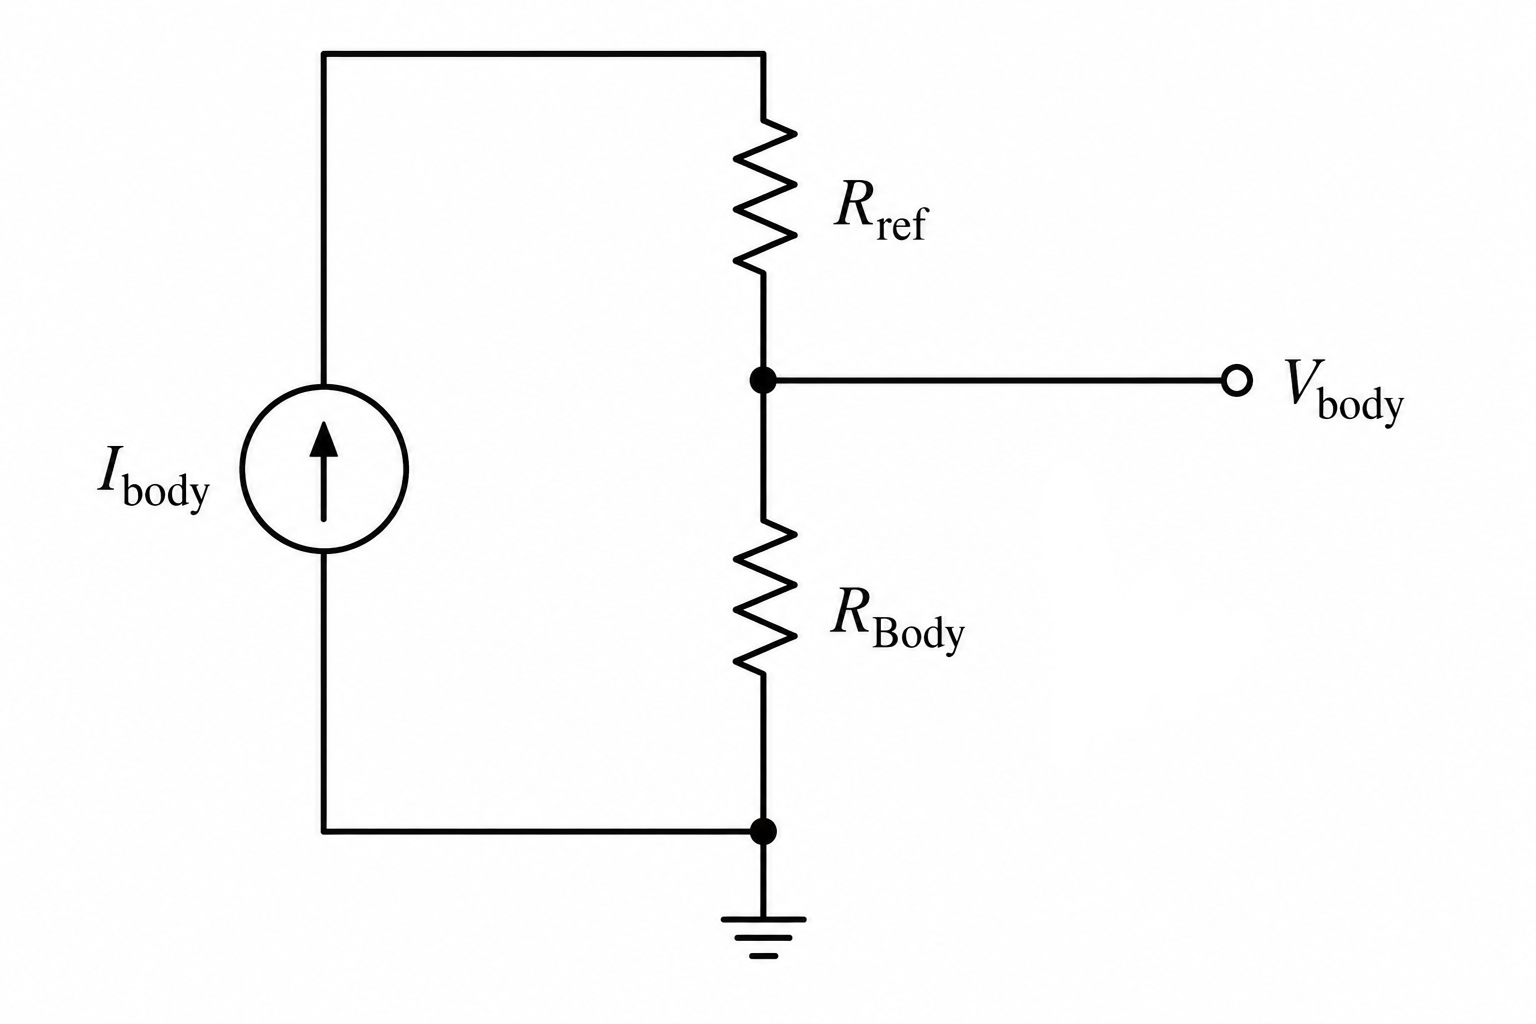
\includegraphics[width=0.5\textwidth]{pics/SP_01.png}
\caption{Medición de resistencia utilizando fuente de corriente constante.
Fuente: elaboración propia.}
\label{fig:ap_fuente_corriente_constante}
\end{figure}

\begin{equation}
R_{body} = \frac{V_{body}}{I_{body}}
\label{eq:ap_resistencia_corriente_constante}
\end{equation}

Por lo tanto, si la corriente aplicada se mantiene constante, la tensión medida
cambia linealmente conforme aumenta o disminuye la resistencia. Esta linealidad
facilita el procesamiento posterior de la señal y reduce la sensibilidad del
resultado frente a pequeños cambios en la tensión medida. La
Figura~\ref{fig:ap_relacion_resistencia_tension_corriente} muestra este
comportamiento.

\begin{figure}[H]
\centering
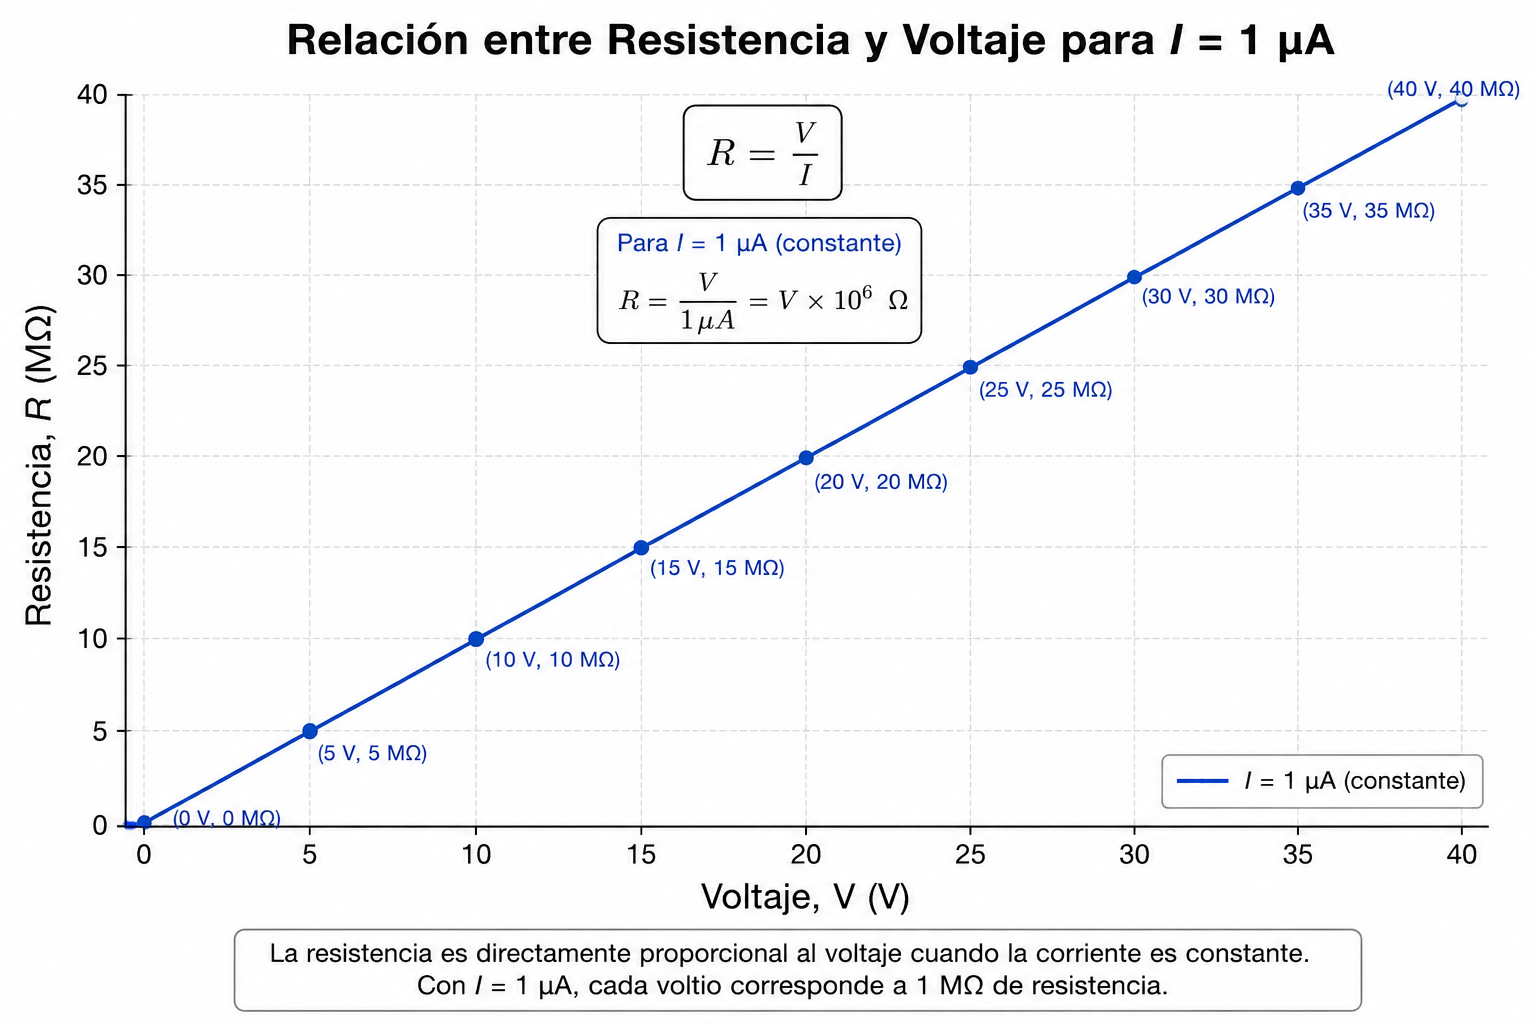
\includegraphics[width=0.75\textwidth]{pics/SP_02.png}
\caption{Relación entre resistencia y tensión medida con corriente
constante. Fuente: elaboración propia.}
\label{fig:ap_relacion_resistencia_tension_corriente}
\end{figure}

Lo anterior convierte al método de corriente constante en un candidato adecuado
para la medición experimental de resistencias de alta impedancia. En cambio, al
analizar el método de tensión constante, se observa que la relación entre la
resistencia y la tensión medida no es lineal. Esto puede provocar que, para
valores altos de resistencia, la sensibilidad de la medición aumente y se pierda
precisión.

El circuito eléctrico equivalente para el método de tensión constante se muestra
en la Figura~\ref{fig:ap_circuito_tension_constante}.

\begin{figure}[H]
\centering
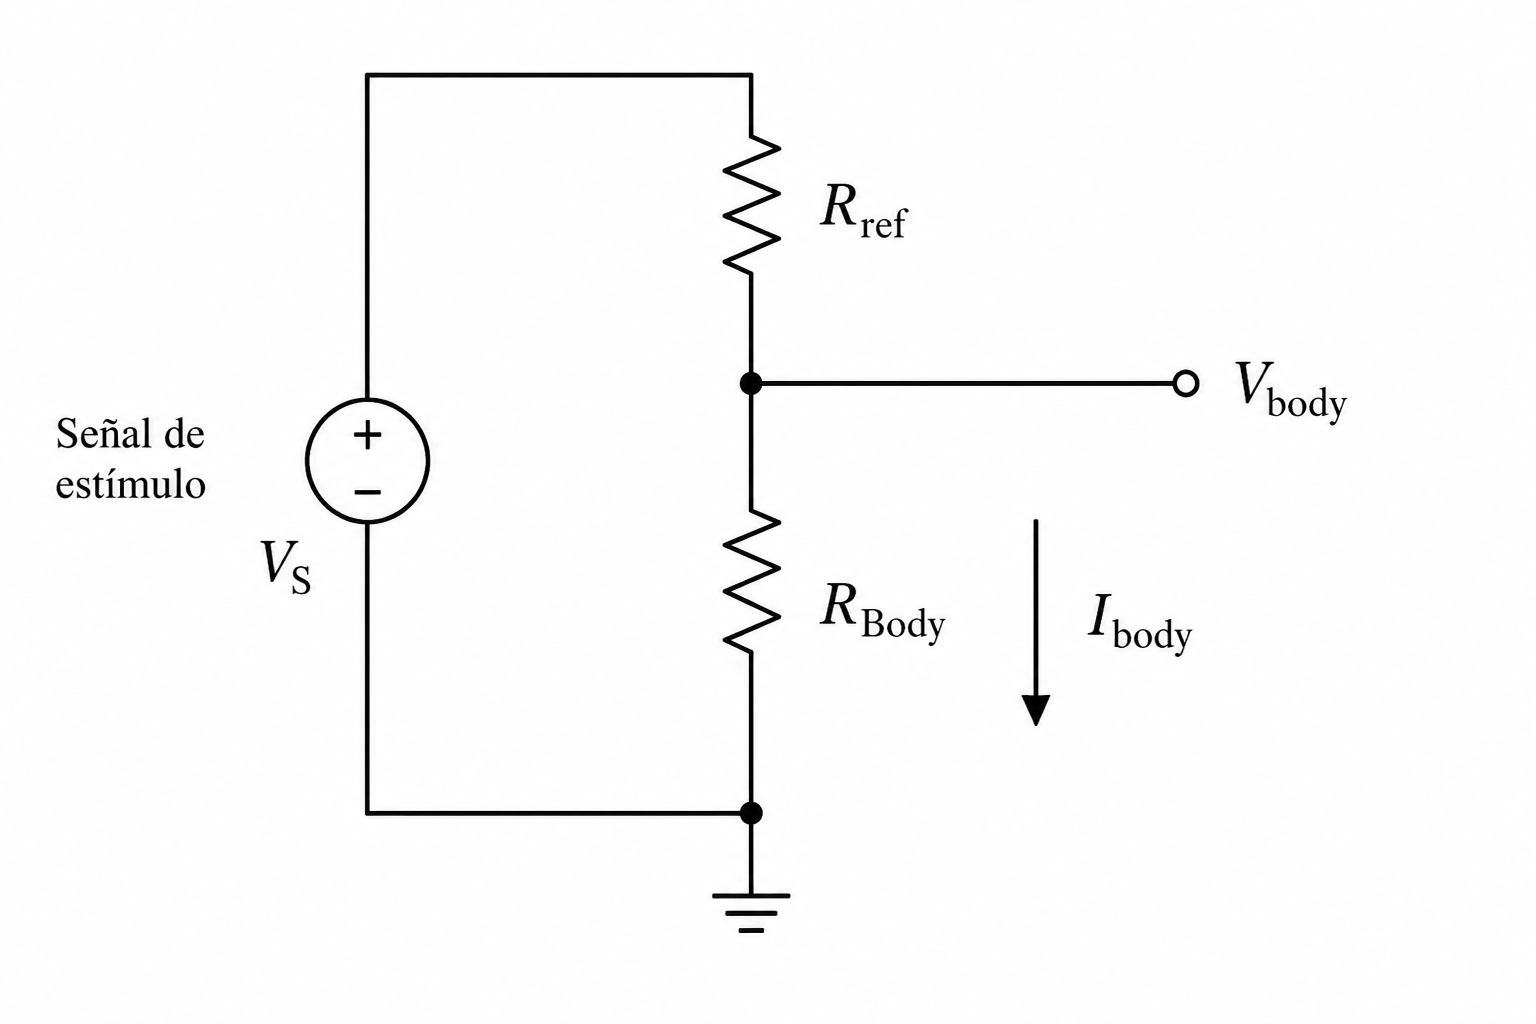
\includegraphics[width=0.75\textwidth]{pics/TF3_4.png}
\caption{Circuito equivalente de medición con fuente de tensión.
Fuente: elaboración propia.}
\label{fig:ap_circuito_tension_constante}
\end{figure}

A partir del circuito anterior, la resistencia del cuerpo puede expresarse como:

\begin{align}
R_{Body} =
\frac{V_{Body} \cdot R_{ref}}{V_{s}-V_{Body}}
\label{eq:ap_resistencia_divisor_tension}
\end{align}

Al graficar la Ecuación~\ref{eq:ap_resistencia_divisor_tension}, se obtiene la
curva mostrada en la Figura~\ref{fig:ap_curva_resistencia_tension}.

\begin{figure}[H]
\centering
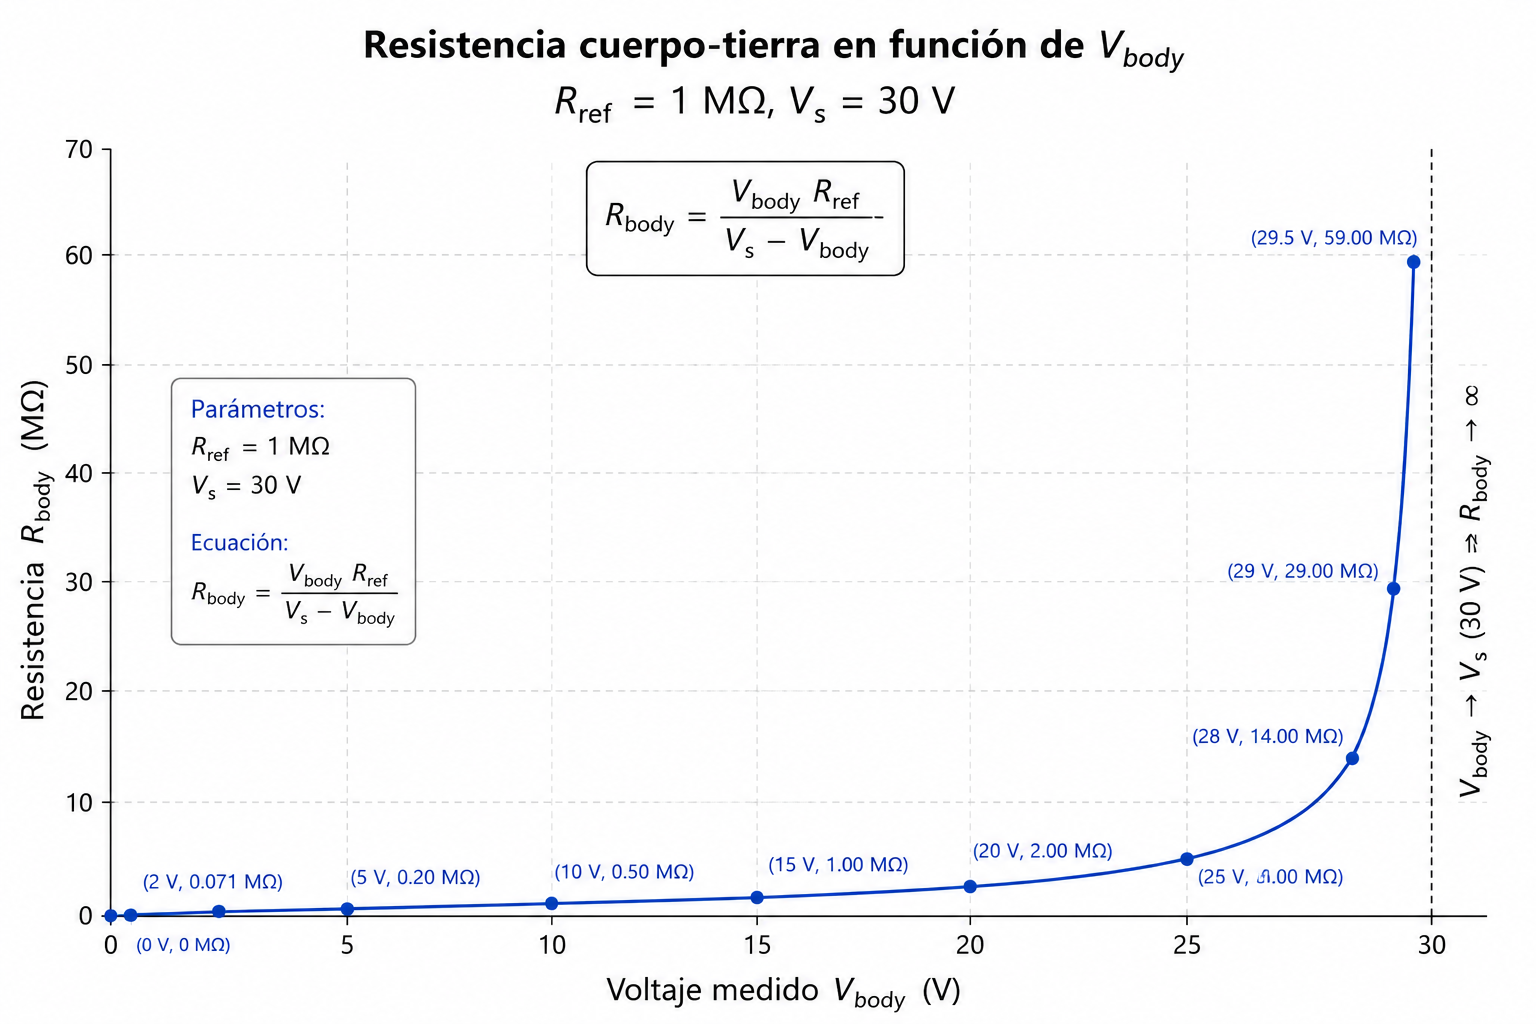
\includegraphics[width=0.75\textwidth]{pics/SP_03.png}
\caption{Comportamiento de $R_{Body}$ con respecto a $V_{Body}$.
Fuente: elaboración propia.}
\label{fig:ap_curva_resistencia_tension}
\end{figure}

Este comportamiento muestra que pequeños cambios en $V_{Body}$ pueden producir
variaciones grandes en la resistencia estimada cuando la tensión medida se
aproxima a $V_s$. Por ejemplo, si $V_{Body}=29.0$ V, se obtiene
$R_{Body}=29$ M$\Omega$. En cambio, si $V_{Body}=29.5$ V, se obtiene
$R_{Body}=59$ M$\Omega$. Para analizar la sensibilidad de la medición, se
calcula la derivada de $R_{Body}$ con respecto a $V_{Body}$, cuyo comportamiento
se muestra en la Figura~\ref{fig:ap_derivada_resistencia_tension}.

\begin{figure}[H]
\centering
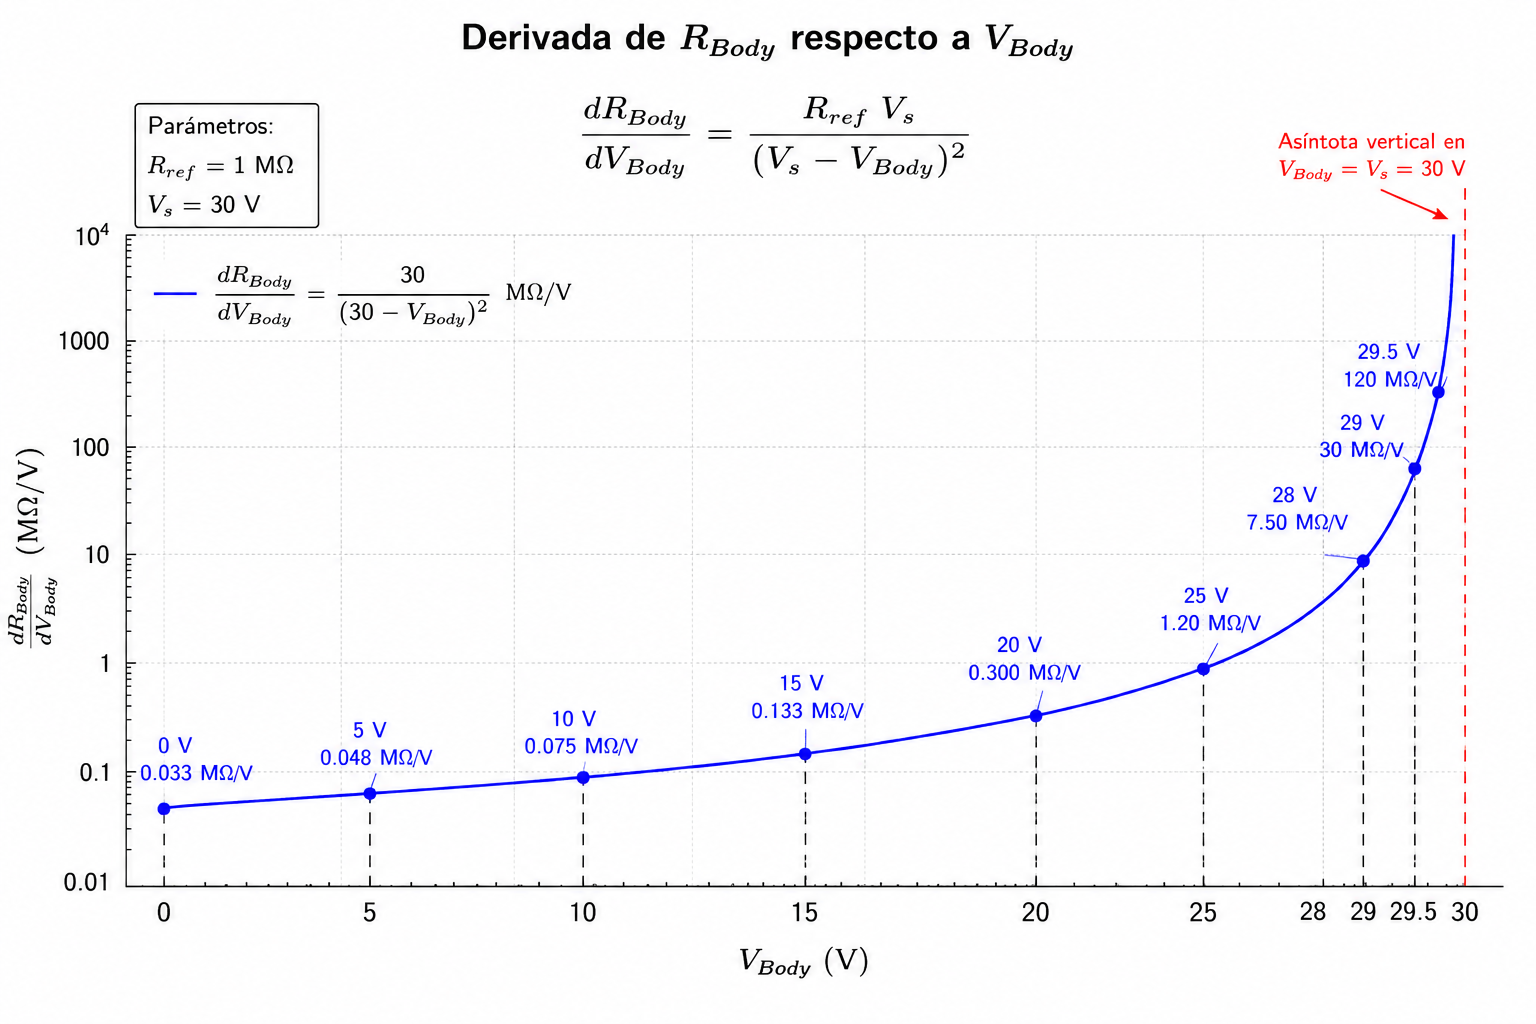
\includegraphics[width=0.75\textwidth]{pics/SP_04.png}
\caption{Comportamiento de la derivada de $R_{Body}$ con respecto a
$V_{Body}$. Fuente: elaboración propia.}
\label{fig:ap_derivada_resistencia_tension}
\end{figure}

Este análisis indica que, en ciertos rangos de operación, una variación de
1 mV puede representar cambios muy grandes en la resistencia estimada. Además,
esta señal debe ser digitalizada. Si se utiliza un ADC de precisión con rango de
medición entre 0 V y 10 V, sería necesario escalar la señal mediante un divisor
de tensión. En consecuencia, el error equivalente en la resistencia aumentaría
desde el punto de vista de la lectura del ADC.

Debido a lo anterior, se selecciona el método de corriente constante para el
diseño experimental. Este método presenta una sensibilidad aproximadamente
constante, lo que permite mantener un comportamiento más uniforme a lo largo del
rango de medición. Además, al controlar la corriente aplicada, es posible
seleccionar un valor suficientemente bajo para reducir la dependencia de
$R_{Body}$ con la tensión aplicada. Para este análisis se considera una corriente
de prueba de 1 $\mu$A.

Una vez definido el método de medición, se plantea un circuito capaz de aplicar
una corriente constante y medir la tensión generada sobre $R_{Body}$. Para la
medición de $V_{Body}$ se propone utilizar un amplificador operacional OPA445,
el cual puede operar con tensiones de alimentación elevadas y presenta una
corriente de polarización del orden de $\pm 100$ pA. En comparación con una
corriente de prueba de 1 $\mu$A, esta corriente representa un error aproximado
de 0.01\%, por lo que su efecto puede considerarse reducido para el alcance del
circuito experimental.

Para la conversión de la señal analógica a digital se propone utilizar un ADC de
precisión AD7606. Este convertidor posee una resolución de 16 bits, permite
trabajar con rangos de entrada de hasta 10 V y utiliza comunicación SPI, lo cual
facilita su integración con un microcontrolador.
